\chapter{The Thick--Client Software--System Architecture of \yerotherpblack}

\vspace{-2em}

\YEROTHCHAPINTRO{
This chapter explains why \yerotherpblack is modular
in its uses, and fits any industrial setting !
}


\vspace{1em}


\begin{table*}[!htbp]
\centering
\resizebox{\textwidth}{!}{%to fit the table within the text width
\begin{tabular}{cccc} 

\multicolumn{1}{c}{}										&
Thick--client application \mycheckmark{yerothColorBlue}		& 
Web--browser--based application								\\ \hline

business code								&
		\yerothvert{user interface}			&						
		\yerothrouge{application server}	\\ \hline
		
co--related software--systems		&
		\yerothvert{$1$ (DBMS)}		&						
		\yerothrouge{at least $3$ (DBMS, web~/~application server)}	\\ \hline
						
number of logical layers									&
		\yerothvert{$2$ (client and data)}					&						
		\yerothrouge{$4$ (client, presentation, logic, and data)}\\ \hline
				
rapid prototyping (\wy tools)		&
		\yerothvert{yes}			&						
		\yerothrouge{very limited}	\\ \hline				
				
software security vulnerability										&
		\yerothvert{low ($1$ programming language)}					&					
		\yerothrouge{high (\emph{several} programming languages)}	\\ \hline

user interface 														&
		\yerothvert{all computers (GUI with \emph{BUSINESS CODE})}	&						
		\yerothvert{all computers (web--browser)}					\\ 		


\end{tabular}}
\caption{Thick--client application VS Web--browser--based application.\\}
\label{tab:TWO-thickclient-application-againts-webbrowserbased-application}
\end{table*}

\vspace{1em}

\section{Business and user interface code deployment}

Table~\ref{tab:TWO-thickclient-application-againts-webbrowserbased-application}
depicts the issue of business and user
interface code deployment on all computers
participating in the functioning of \yerotherpblack,
as a software--system for a user.

We tackle the problem of automatic deployment of
business and user interface code on all user
computers by using the '\texttt{apt upgrade}'
software--system on '\debianlinux'.


\section{Databases}

DBMS \MySQL is used for storing and managing huge
data accross globe.

\section{NUMBER OF LOGICAL SOFTWARE--SYSTEM LAYERS: E.G. Sample technical configurations}

This section illustrates $2$ different possible
computer network configurations that
could prevail in industry. 

\newpage

\subsection{Sample $2$--computers store}

\begin{center}
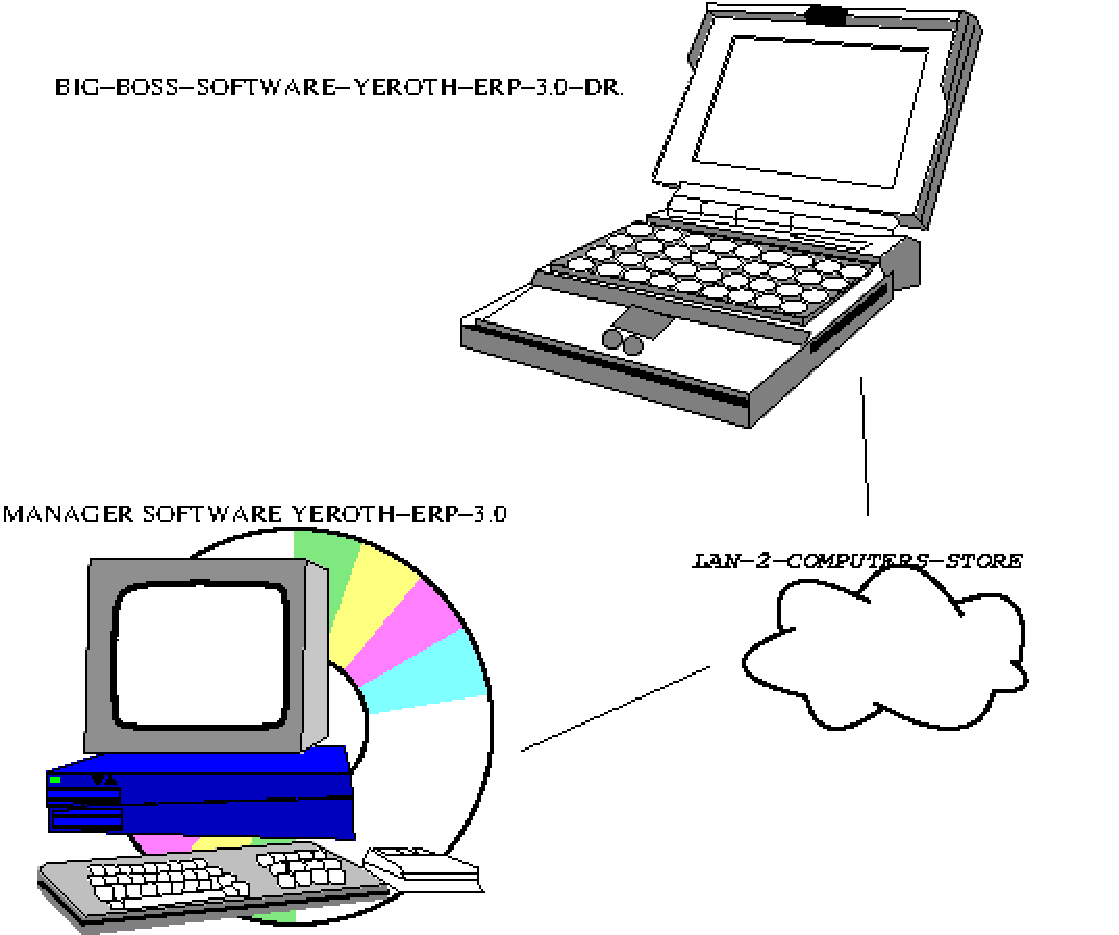
\includegraphics[scale=0.7]{images/yeroth-erp-sample-2-computers-store.pdf}
\captionof{figure}{Sample $2$--computers store.}
\label{fig:sample-two-computers-store}
\end{center}
\index{Sample $2$--computers store}

\newpage

\subsection{Sample decentralized multi sites supermarket}

\begin{center}
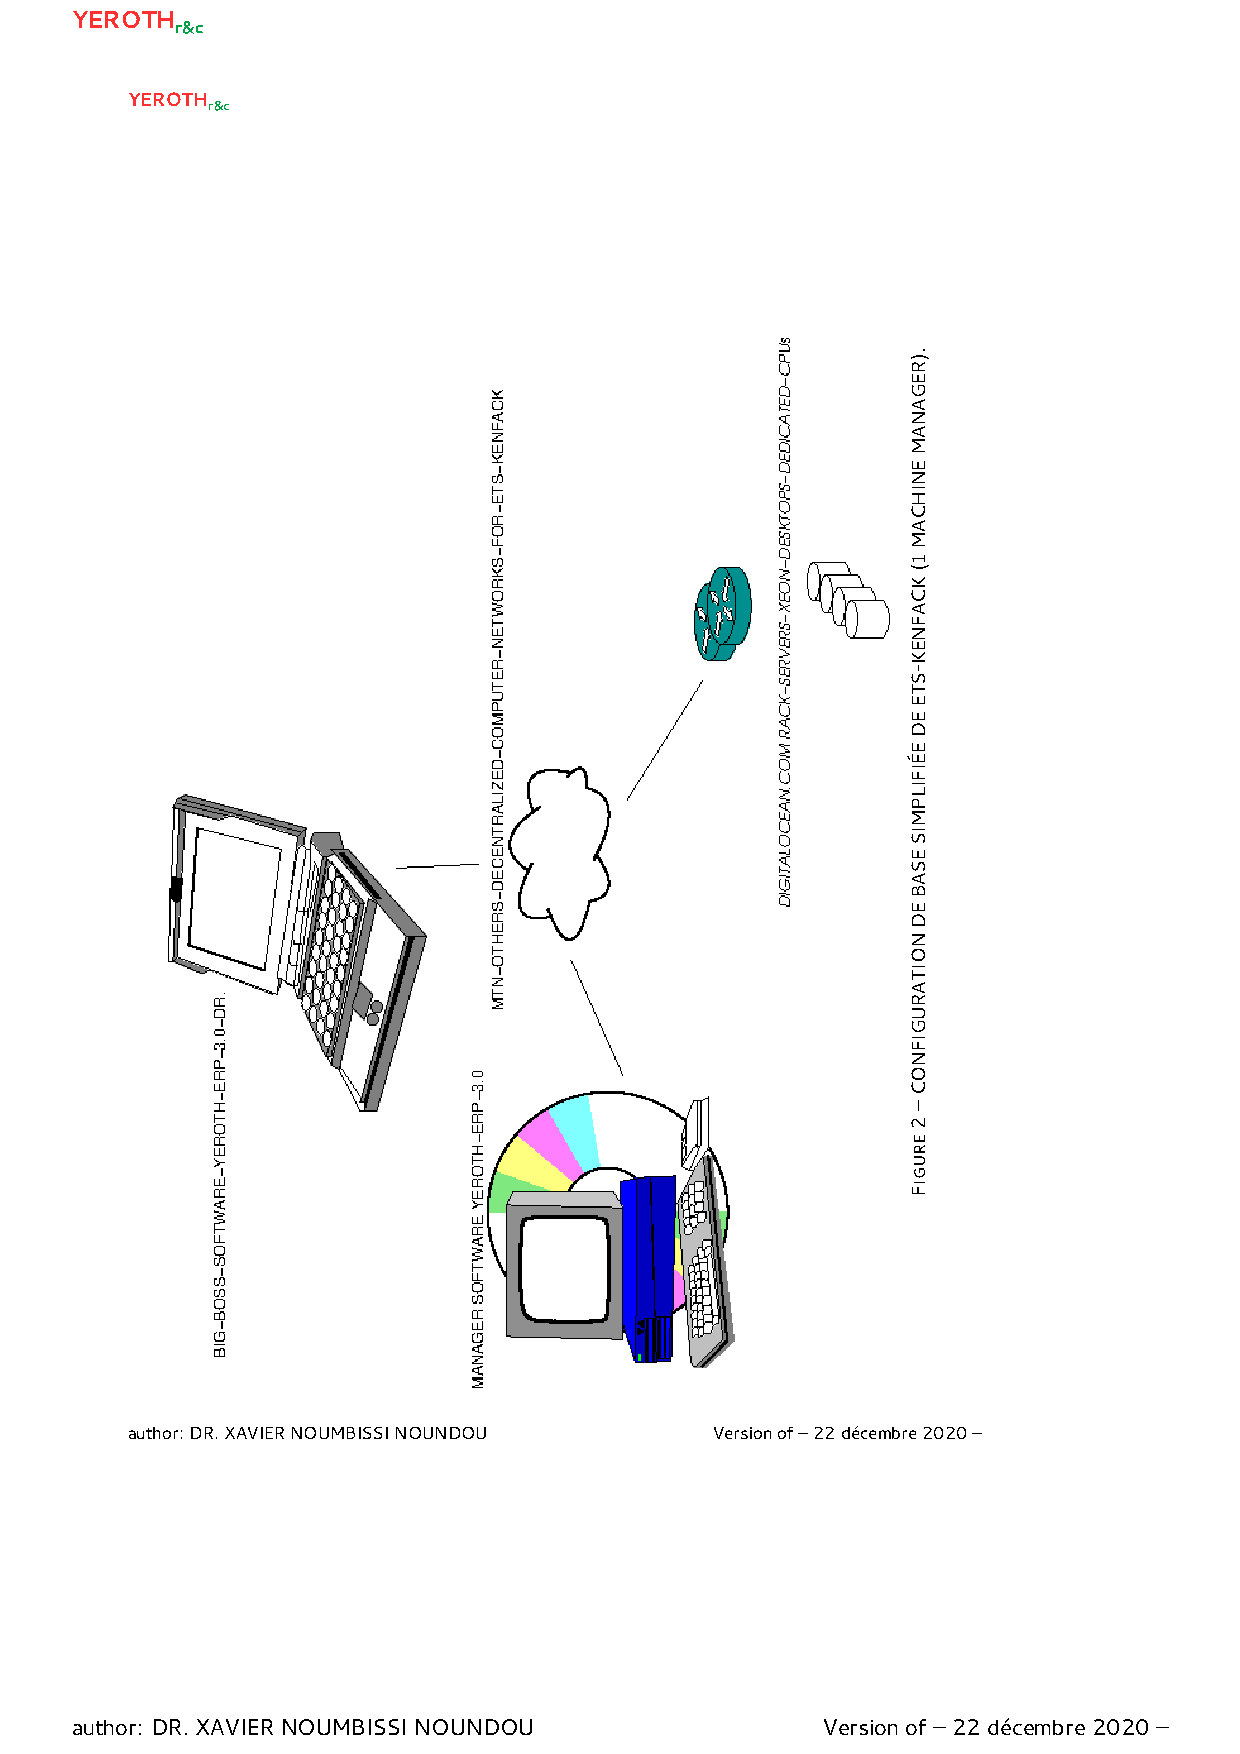
\includegraphics[scale=0.81]{images/yeroth-sample-decentralized-multi-sites-supermarket.pdf}
\captionof{figure}{Sample decentralized multi sites supermarket.}
\label{fig:sample-decentralized-multi-sites-supermarket}
\end{center}
\index{sample decentralized multi sites supermarket}

\newpage

\section{Software Security Vulnerability in YEROTH--ERP--3.0}
\index{software security vulnerability}

I perform security vulnerability detection for open source
software \yerotherpblack by using memory leak detection
tool 'valgrind~\cite{conf:pldi:NethercoteS07}'.
